\section{Part 1}
\subsection*{Formulas}
\[\sum_{i=0}^{n-1} ar^i = \frac{a(1-r^n)}{1-r}\]
For given rate $r\%$ over time period $t\in[0, T]$,
with annual period $P$,
discount factor $d_{0,T}$ is given
\[d_{0,T} = \left(1+r\% \times \frac{T}{P}\right)^{-1} < 1\]
\subsection*{No Arbitrage Argument}
To prove $A=B$, show strategies for $A\neq B$.
If $A>B$, short on $A$, long on $B$, and vice versa.
\subsection*{1.1.2 Asset w/ Predictable Income}
\[F_0 = (S_0-C)/d_{0,T}, where C = C'd_{0,t}\]
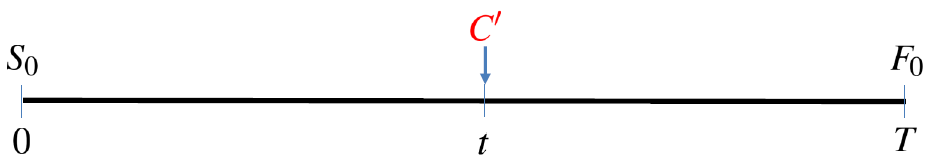
\includegraphics[width=\linewidth]{contents/1.1.2.png}
\subsection*{1.1.3 Asset w/ Continuous Dividend Yield}
Annualized continuous dividend yield of $q$
\[F_0=S_0\exp((r-q)T)\]
\subsection*{1.1.4 Asset w/ Storage Costs}
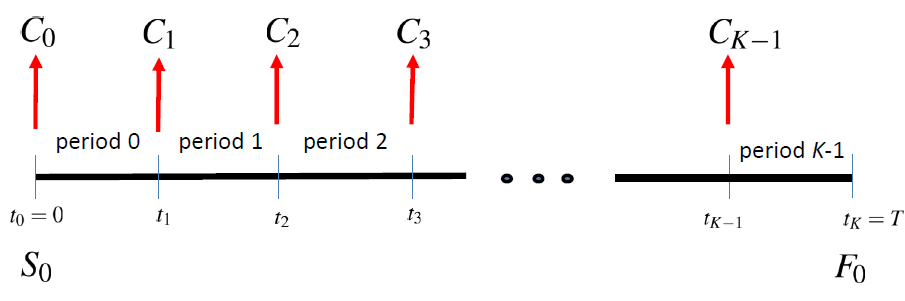
\includegraphics[width=\linewidth]{contents/1.1.4.png}
\[d_{0,K} F_0 = S_0 + \sum_{j=0}^{K-1}d_{0,j}C_j\]
\subsection*{1.1.5 Convenience Yield}
\[d_{0,K} F_0 = S_0 + \sum_{j=0}^{K-1}d_{0,j}(C_j-y)\]
\subsection*{1.2 Value of Forward}
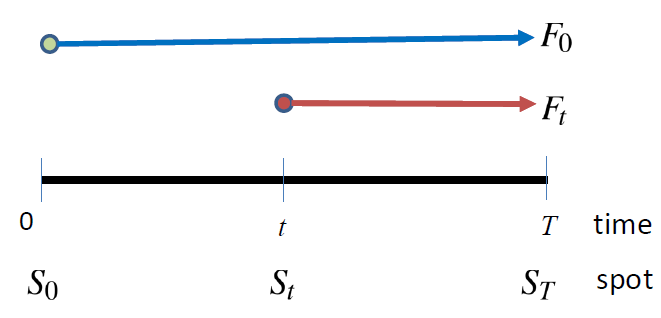
\includegraphics[width=\linewidth]{contents/1.2.png}
\[f_t = (F_t-F_0)d_{t,T}\]
